\begin{problem}{Rebuild}{standard input}{standard output}{1s}{light green}

Archaeologists find ruins of Ancient ACM Civilization, and they want to rebuild it.

The ruins form a closed path on an x-y plane, which has $n$ endpoints.
The endpoints locate on $(x_1,y_1)$, $(x_2,y_2)$, $\ldots,(x_n,y_n)$ respectively.
Endpoint $i$ and endpoint $i-1$ are adjacent for $1<i\leq n$, also endpoint $1$ and endpoint $n$ are adjacent.
Distances between any two adjacent endpoints are positive integers.

To rebuild, they need to build one cylindrical pillar at each endpoint, the radius of the pillar of endpoint $i$ is $r_i$.
All the pillars perpendicular to the x-y plane, and the corresponding endpoint is on the centerline of it.
We call two pillars are adjacent if and only if two corresponding endpoints are adjacent.
For any two adjacent pillars, one must be tangent externally to another, 
otherwise it will violate the aesthetics of Ancient ACM Civilization.
If two pillars are not adjacent, then there are no constraints, even if they overlap each other.

Note that $r_i$ must not be less than $0$ since we cannot build a pillar with negative radius 
and pillars with zero radius are acceptable since those kind of pillars still exist in their neighbors.

You are given the coordinates of $n$ endpoints. Your task is to find $r_1,r_2,\ldots,r_n$ which makes sum of base area of all pillars as minimum as possible.

\def\ll{0.2}
\begin{center}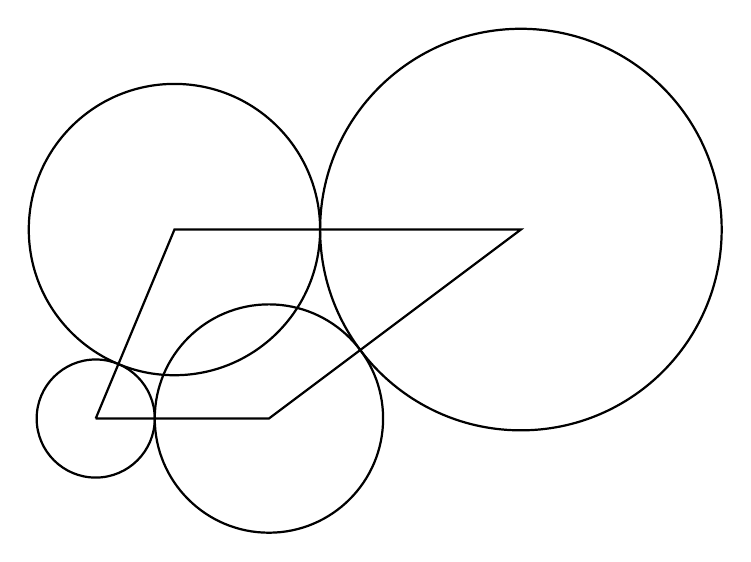
\begin{tikzpicture}[my node/.style={circle,fill=black}]
\draw[thick] ( 0*\ll, 0*\ll) -- (11*\ll, 0*\ll) -- (27*\ll,12*\ll) -- ( 5*\ll,12*\ll) -- ( 0*\ll, 0*\ll);
\draw[thick] ( 0*\ll, 0*\ll) circle ( 3.75*\ll);
\draw[thick] (11*\ll, 0*\ll) circle ( 7.25*\ll);
\draw[thick] (27*\ll,12*\ll) circle (12.75*\ll);
\draw[thick] ( 5*\ll,12*\ll) circle ( 9.25*\ll);
\end{tikzpicture} \\
Example
\end{center}



For example, if the endpoints are at $(0,0)$, $(11,0)$, $(27,12)$, $(5,12)$, we can choose ($r_1$, $r_2$, $r_3$, $r_4$)$=$($3.75$, $7.25$, $12.75$, $9.25$).
The sum of base area equals to $3.75^2\pi+$$7.25^2\pi+12.75^2\pi+9.25^2\pi=988.816\ldots$. 
Note that we count the area of the overlapping parts multiple times.

If there are several possible to produce the minimum sum of base area, you may output any of them.

\InputFile
The first line contains an integer $t$ indicating the total number of test cases.
The following lines describe a test case.

The first line of each case contains one positive integer $n$, the size of the closed path.
Next $n$ lines, each line consists of two integers $(x_i,y_i)$ indicate the coordinate of the $i$-th endpoint.
\begin{itemize}
\item $1 \le t \le 100$
\item $3 \le n \le 10^4$
\item $|x_i|,|y_i|\leq 10^4$
\item Distances between any two adjacent endpoints are positive integers.
\end{itemize}

\pagebreak
\OutputFile
If such answer doesn't exist, then print on a single line "IMPOSSIBLE" (without the quotes). 
Otherwise, in the first line print the minimum sum of base area, 
and then print $n$ lines, the $i$-th of them should contain a number $r_i$, 
rounded to 2 digits after the decimal point.

If there are several possible ways to produce the minimum sum of base area, you may output any of them.

\Example

\begin{example}
\exmp{
3
4
0 0
11 0
27 12
5 12
5
0 0
7 0
7 3
3 6
0 6
5
0 0
1 0
6 12
3 16
0 12
}{
988.82
3.75
7.25
12.75
9.25
157.08
6.00
1.00
2.00
3.00
0.00
IMPOSSIBLE
}%
\end{example}
\end{problem}